% sample.tex — fixture PDF for the Ship of Tools preview pane.
% A short, real technical note: multi-page layout, display mathematics, a
% vector (TikZ) figure, and a table. Build: pdflatex sample.tex (twice, for
% the figure cross-reference). Kept to three pages for the pagination demo.
\documentclass[11pt]{article}
\usepackage[margin=1in]{geometry}
\usepackage{amsmath,amssymb}
\usepackage{booktabs}
\usepackage{xcolor}
\usepackage{tikz}
\usetikzlibrary{angles,quotes,calc}

\definecolor{sotgreen}{HTML}{389826}
\definecolor{sotpurple}{HTML}{9558B2}
\definecolor{sotred}{HTML}{CB3C33}

\newcommand{\hav}{\operatorname{hav}}

\title{\textbf{Great-Circle Distance on a Sphere}\\[2pt]
  \normalsize A short worked note}
\author{\textsl{Ship of Tools} — preview sample}
\date{}

\begin{document}
\maketitle
\thispagestyle{empty}

\begin{abstract}
\noindent The shortest path between two points on a sphere follows a
\emph{great circle}. This note collects the two standard formulae — the
spherical law of cosines and the numerically stable haversine — and works a
small four-waypoint route as an example. It doubles as a preview fixture,
exercising multi-page layout, display mathematics, a vector figure, and a
table.
\end{abstract}

\section{Setup}
Let two points on a sphere of radius $R$ have latitudes $\phi_1,\phi_2$ and
longitudes $\lambda_1,\lambda_2$, and write the differences
\[
  \Delta\phi = \phi_2-\phi_1, \qquad \Delta\lambda = \lambda_2-\lambda_1 .
\]
The central angle $\theta$ subtended at the sphere's centre fixes the arc
length through $d = R\,\theta$; everything below is a way to get $\theta$ from
the coordinates.

\section{The central angle}
The spherical law of cosines gives it directly,
\[
  \cos\theta = \sin\phi_1\sin\phi_2
             + \cos\phi_1\cos\phi_2\cos\Delta\lambda ,
\]
but for nearly-coincident points this form loses precision to floating-point
cancellation. The \emph{haversine} identity avoids it:
\[
  \hav(\theta) = \hav(\Delta\phi)
    + \cos\phi_1\cos\phi_2\,\hav(\Delta\lambda),
  \qquad \hav(x) = \sin^2\!\tfrac{x}{2},
\]
which rearranges to the working formula
\[
  \boxed{\,d = 2R \arcsin\sqrt{\,\sin^2\!\frac{\Delta\phi}{2}
    + \cos\phi_1\cos\phi_2\,\sin^2\!\frac{\Delta\lambda}{2}}\,}.
\]

\newpage

\section{Geometry}
Figure~\ref{fig:gc} fixes the picture: the great-circle arc (green) is the
distance we want, $d = R\theta$; the straight chord (dashed) is the shorter
Euclidean distance through the interior and is \emph{not} what a traveller on
the surface covers.

\begin{figure}[h]
\centering
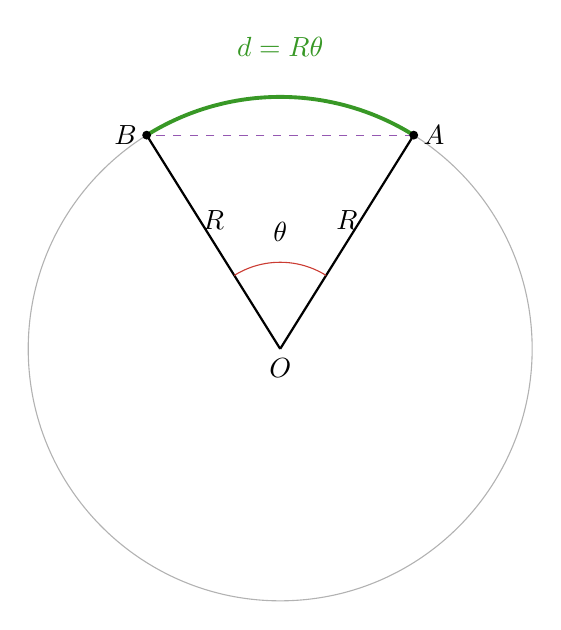
\begin{tikzpicture}[scale=3.2,>=latex]
  \coordinate (O) at (0,0);
  \coordinate (A) at (58:1);
  \coordinate (B) at (122:1);
  \draw[gray!60] (O) circle (1);
  \draw[thick] (O) -- (A);
  \draw[thick] (O) -- (B);
  \draw[sotgreen, line width=1.4pt] (58:1) arc (58:122:1);
  \draw[dashed, sotpurple] (A) -- (B);
  \pic[draw=sotred, angle radius=11mm, angle eccentricity=1.35,
       "$\theta$"] {angle=A--O--B};
  \node[below] at (O) {$O$};
  \node[above=1pt] at ($(O)!0.5!(A)$) {$R$};
  \node[above=1pt] at ($(O)!0.5!(B)$) {$R$};
  \fill (A) circle (0.5pt); \node[right] at (A) {$A$};
  \fill (B) circle (0.5pt); \node[left]  at (B) {$B$};
  \node[sotgreen] at (90:1.2) {$d = R\theta$};
\end{tikzpicture}
\caption{Two surface points $A,B$ on a sphere of radius $R$. The great-circle
distance is the arc $d = R\theta$, with $\theta$ the central angle at $O$; the
dashed chord is the shorter straight-line distance.}
\label{fig:gc}
\end{figure}

\noindent Because $\theta \le \pi$ for the minor arc, $\arcsin$ returns the
correct branch and the haversine formula needs no quadrant bookkeeping — one
reason it is the default in practice.

\newpage

\section{A worked route}
Take a four-waypoint route across northern New Mexico and sum the legs on a
spherical Earth, $R = 6371~\mathrm{km}$. Table~\ref{tab:route} lists each leg
from the working formula above.

\begin{table}[h]
\centering
\begin{tabular}{llr}
\toprule
From & To & Leg (km) \\
\midrule
Albuquerque & Santa Fe   & 93.5 \\
Santa Fe    & Black Mesa  & 23.7 \\
Black Mesa  & Taos       & 75.5 \\
\midrule
\multicolumn{2}{l}{\textbf{Total}} & \textbf{192.7} \\
\bottomrule
\end{tabular}
\caption{Per-leg great-circle distances for the demo route; the total,
$192.7~\mathrm{km}$, is what \texttt{route\_length} returns in the demo
project.}
\label{tab:route}
\end{table}

\noindent The same computation lives in the demo project as
\texttt{route\_length}, dispatched over a vector of \texttt{Waypoint}s — the
figure it plots and this table are two views of one function.

\vfill
\noindent\rule{\linewidth}{0.4pt}\\[2pt]
{\small References: Sinnott, R.~W. (1984), \emph{Virtues of the Haversine},
Sky \& Telescope \textbf{68}(2), 159. — Vincenty, T. (1975), \emph{Direct and
inverse solutions of geodesics on the ellipsoid}.}

\end{document}
